\begin{titlepage}
\begin{flushleft}

% Logos
\noindent\begin{minipage}[t]{0.49\textwidth}
	\begin{flushleft}
		\vspace{0pt} %needed else aligned to bottom
		
\includegraphics[width=200px]{./images/logo-hsr}
	\end{flushleft}
\end{minipage}
\hfill
\begin{minipage}[t]{0.49\textwidth}
	\begin{flushright}
		\vspace{0pt} %needed else aligned to bottom
		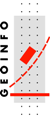
\includegraphics[width=40px]{./images/logo-geoinfo}
	\end{flushright}
\end{minipage}
\\[1.5cm]

% Title
\fbox{
	\parbox{\dimexpr \linewidth - 2\fboxrule - 2\fboxsep}{
		\begin{center}
			\Large \bfseries Cloudbasiertes Geodatenmanagement mit Google Fusion Tables: Entwicklung eines Cloud-GIS Prototypen
		\end{center}
	}
}
\\[1.5cm]

% Arbeitstyp / Schule
\begin{center}
{\Large \bfseries Studienarbeit}\\[0.5cm]
{\Large
	Abteilung Informatik \\[0.2cm]
	Hochschule für Technik Rapperswil
}\\[1.5cm]
\end{center}

% Semester
\fbox{
	\parbox{\dimexpr \linewidth - 2\fboxrule - 2\fboxsep}{
		\begin{center}
			\Large Frühjahrssemester 2012
		\end{center}
	}
}
\\[1.5cm]

\begin{tabular}{lp{12cm}}
Autoren: & \textbf{Stefan Oderbolz} (\url{soderbol@hsr.ch}) \newline
 \textbf{Jürg Hunziker} (\url{jhunzike@hsr.ch}) \\ 
Betreuer: & \textbf{Prof S. Keller} (\url{sfkeller@hsr.ch}) \\ 
Projektpartner: & \textbf{Marco Lehmann}, GEOINFO AG Herisau, \url{http://www.geoinfo.ch} \\ 
Experte: & \textbf{Prof S. Keller} (\url{sfkeller@hsr.ch}) \\ 
Datum: & \textbf{29. Mai 2012} \\ 
\end{tabular}

\end{flushleft}
\end{titlepage}
